\section{Rapport de fin d'itération}
Un des objectifs primaires de cette itération était de peaufiner le programme 
dans son ensemble; outre celui d'implémenter l'histoire 6 - Statistiques.
Cet objectif a été atteint, selon nos standards. Nous sommes fierté, nous sommes
bonheur et HomePlans est un logiciel de type sympathique dont la simplicité
d'utilisation créera une nouvelle génération d'architectes heureux de pouvoir
exprimer leur créativité dans un environnement libre de contraintes et, très
probablement, de bugs.

\subsection{Follow-up sur le rapport de fin d'itération précédente}

	\paragraph{Analyse de la classe Ordered}
	Nous avons donc compris plus tard que ce qui posait problème avec la classe
	Ordered était le sens sémantique de cette dernière. Comme un étage n'est pas
	en lui-même ordonné, mais plutôt indexé dans la liste des étages, nous avons
	renommé la classe \texttt{Ordered} en \texttt{Indexed}.

	\paragraph{Optimisation des objets importés}
	Ce problème a été adressé, et une meilleure description de la solution sera
	donnée infra.
	
	\paragraph{Finition}
	Très clairement, la logique d'utilisation a été largement améliorée, notamment
	grâce à certains rajouts (construction des murs en live, snap to grid,...) et
	aussi à la réimagination de la sélection.
	

\subsection{Suivi du planning}
Pour cette dernière itération, nous avons aussi réussi à atteindre tous nos 
objectifs. Nous notons toutefois que ce fut le cas pour toutes les itérations
jusqu'ici, soyons-en donc heureux.

\subsection{Librairies introduites}

	\paragraph{JDelaunay}
	La manière dont nous reliions tous les points d'un sol était naïve et pouvait
	être largement améliorée. Nous avons décidé d'utiliser la triangulation de 
	Delaunay; ce qui permet notamment de dessiner des pièces concaves dans la 
	joie la plus totale.

	JDelaunay était le choix sensible comme librairie à importer pour ce dessein,
	étant disponible sur GitHub avec une documentation suffisante : facile à 
	utiliser, facile à installer. 

\subsection{Architecture}

	\subsubsection{Statistiques}
	Deux classes ont été rajoutées pour prendre en charge le traitement des
	statistiques : \texttt{StatisticsController}, \texttt{StatisticsView}, dans
	le modèle MVC. Nous avons bien entendu dû rajouter quelques fonctions dans
	le modèle liées au calcul desdites statistiques.

	\subsubsection{Factory export}
	Comme promis lors de la troisième démonstration, nous avons aussi appliqué
	l'architecture Factory au module d'export d'objets. Il l'était déjà pour le
	module d'import. La nouvelle architecture est présentée en figure \ref{fig:archi:exportfactory}
	\begin{figure}
		\center
		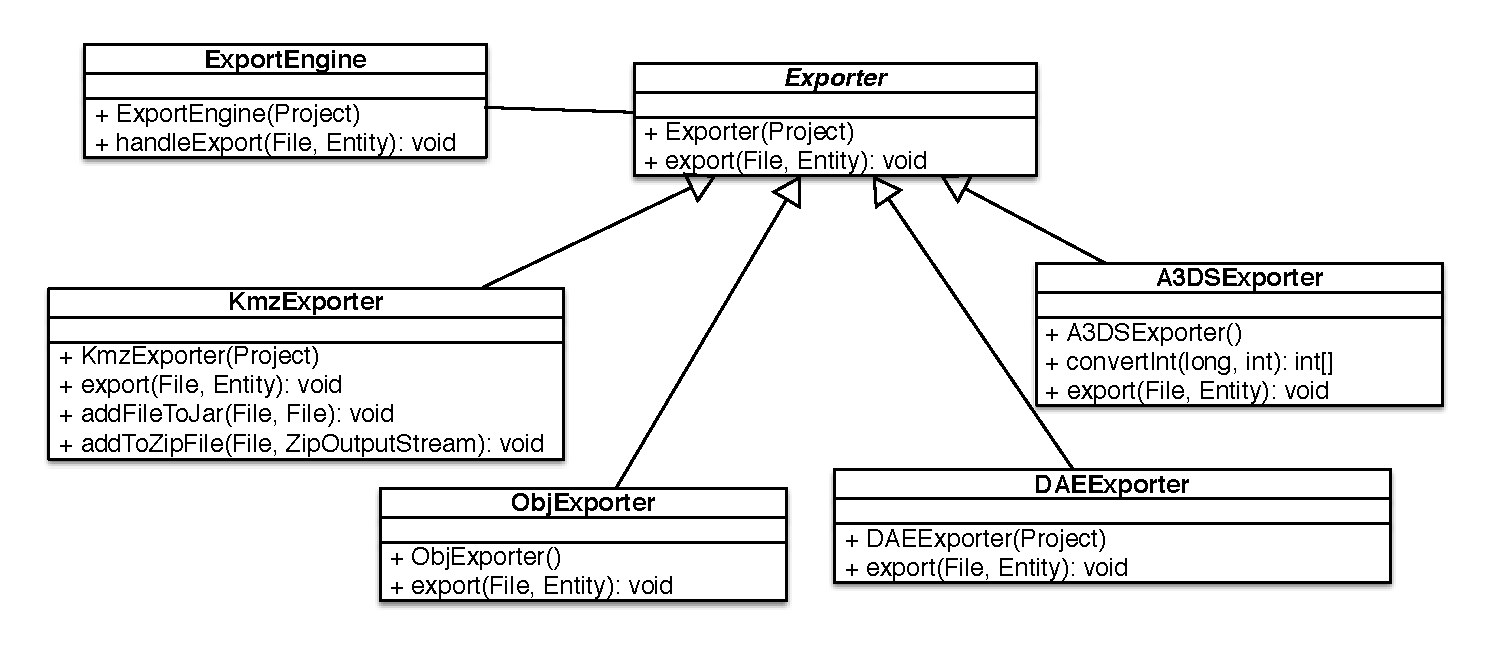
\includegraphics[width=\textwidth]{iteration4/fig/exportfactory.eps}
		\caption{\label{fig:archi:exportfactory} Architecture du système d'export}
	\end{figure}

	\subsubsection{Sélection}
	Nous avons décidé de changer la manière dont la sélection d'objets et de
	pièces fonctionne. Avant, il était possible de sélectionner plusieurs objets
	en même temps et cela causait des problèmes de logique, notamment pour les 
	statistiques où nous devions présenter les statistiques de l'unique pièce 
	sélectionnée.

	Nous avons donc déplacé la logique de la sélection dans une classe, le 
	\texttt{SelectionManager}, y compris la logique de l'étage courant.

	Le \texttt{SelectionManager} s'assure que toutes les contraintes suivantes
	sont respectées : 
	\begin{itemize}
		\item maximum une pièce est sélectionnée
		\item maximum un objet est sélectionné
		\item maximum une primitive est sélectionnée
		\item une pièce, un objet et une primitive ne peuvent être sélectionnés ensemble
		\item l'étage courant est l'étage sur lequel se trouvait le dernier objet sélectionné
	\end{itemize}

	De plus, il permet d'accéder à l'objet couramment sélectionné. Il est possible
	de voir comment cette classe s'intègre au reste de l'architecture sur les schémas
	d'architecture finaux.

\subsection{Changements}

	\subsubsection{Construction des murs en live}
	Nous voyons désormais les murs se construire en jaune lorsqu'on crée une
	nouvelle pièce, pour mieux visualiser la nouvelle construction.

	\subsubsection{Déplacement plus rapide des objets}
	Jadis, tout déplacement en cours (lorsque l'utilisateur glisse son clic) d'objet
	dans la vue 3D provoquait une écriture de la nouvelle position de l'objet dans
	la base de données afin de notifier les différents composants de l'application.

	Cependant, l'enregistrement n'est réellement nécessaire que lorsque l'objet
	est placé à sa position finale.

	Désormais, le contrôleur ne notifie que la vue lors du déplacement de l'objet,
	puis tous les différents composants une fois que l'objet a été déposé.

	Cela résulte en une drastique amélioration des performances.

	\subsubsection{Snap to grid}
	Si l'utilisateur presse sur "Shift" lorsqu'il place des points ou déplace
	des objets ou des points, le déplacement est locké à la grille.

\subsection{Bonnes pratiques - Outils}

	\paragraph{Tests unitaires}
	Dans les dernières heures de la dernière itération, nous avons effectué un 
	très petit changement qui améliorait les performances. Tragiquement, un de nos
	fiables et nombreux tests unitaires ne passait plus; nous avons dès lors 
	pris la décision de désactiver ce changement et nous sommes rendus compte plus
	tard que nous nous heurtions à des comportements inattendus. Merci le test 
	unitaire donc!

\subsection{Diagrammes de classes finaux}

	\subsubsection{Package Models}
	\begin{figure}[!H]
		\center
		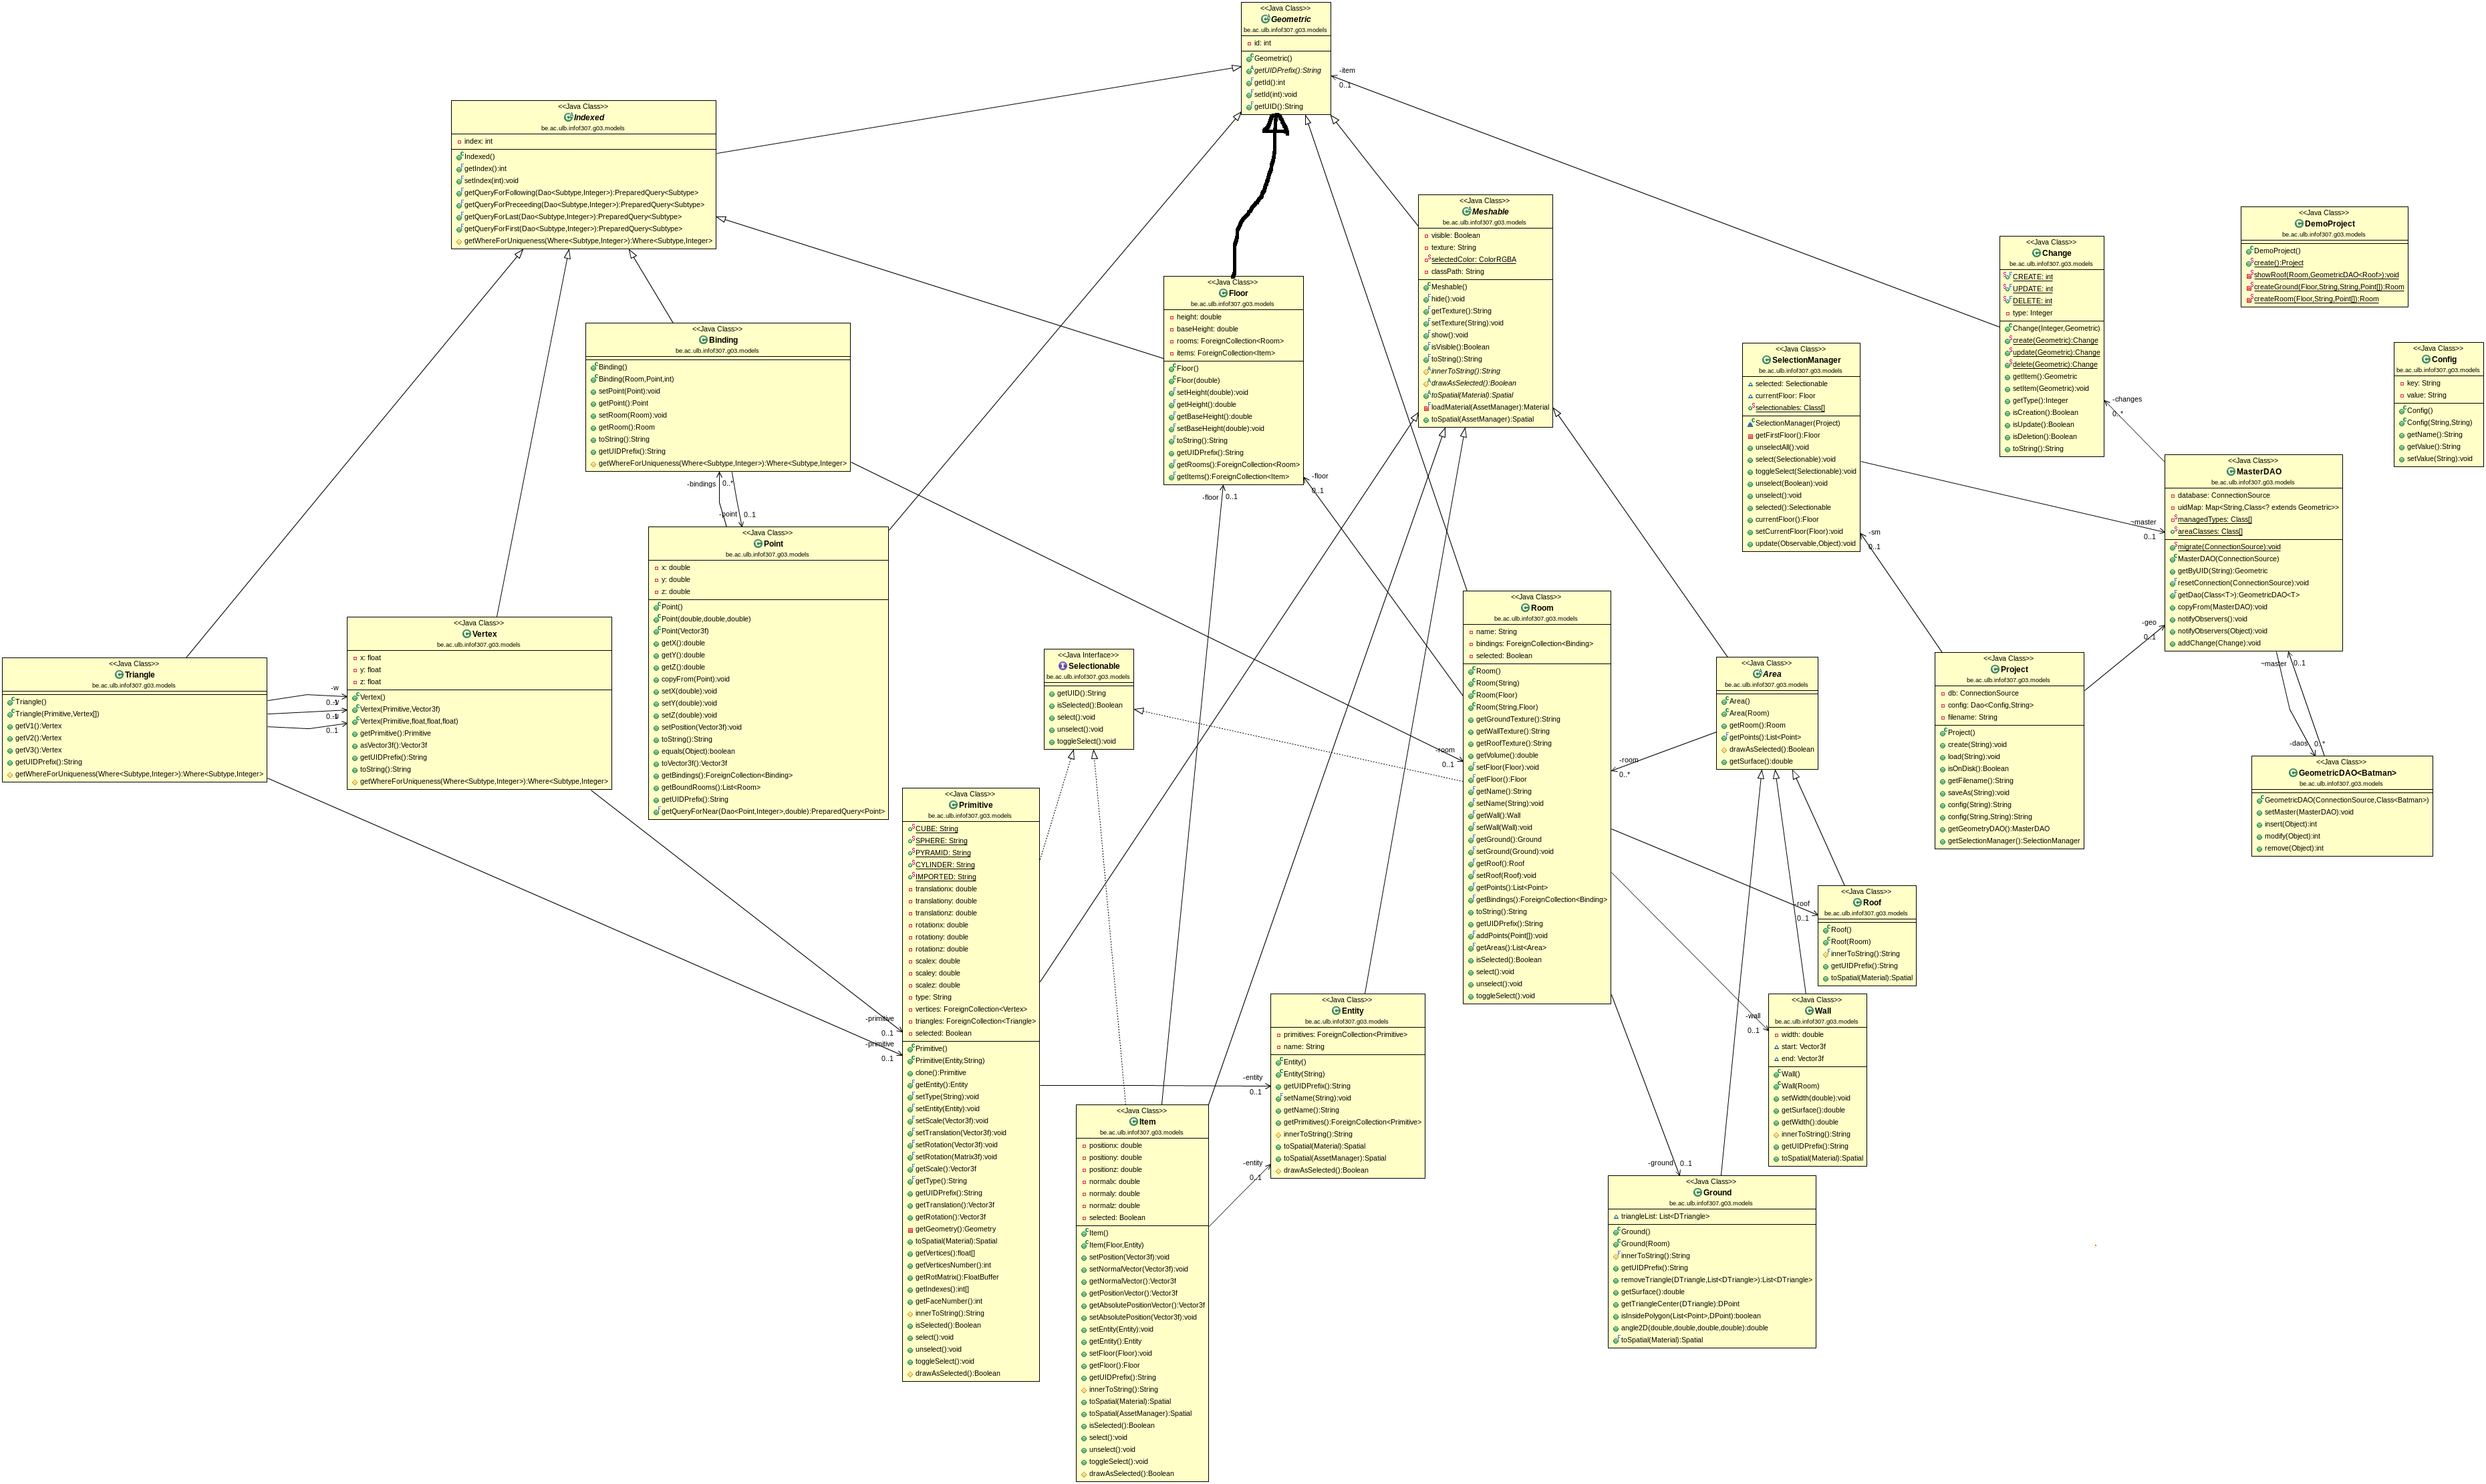
\includegraphics[width=\textwidth]{iteration4/fig/models-final-hand.png}
	\end{figure}

	\subsubsection{Package GUI}
	\begin{figure}[!H]
		\center
		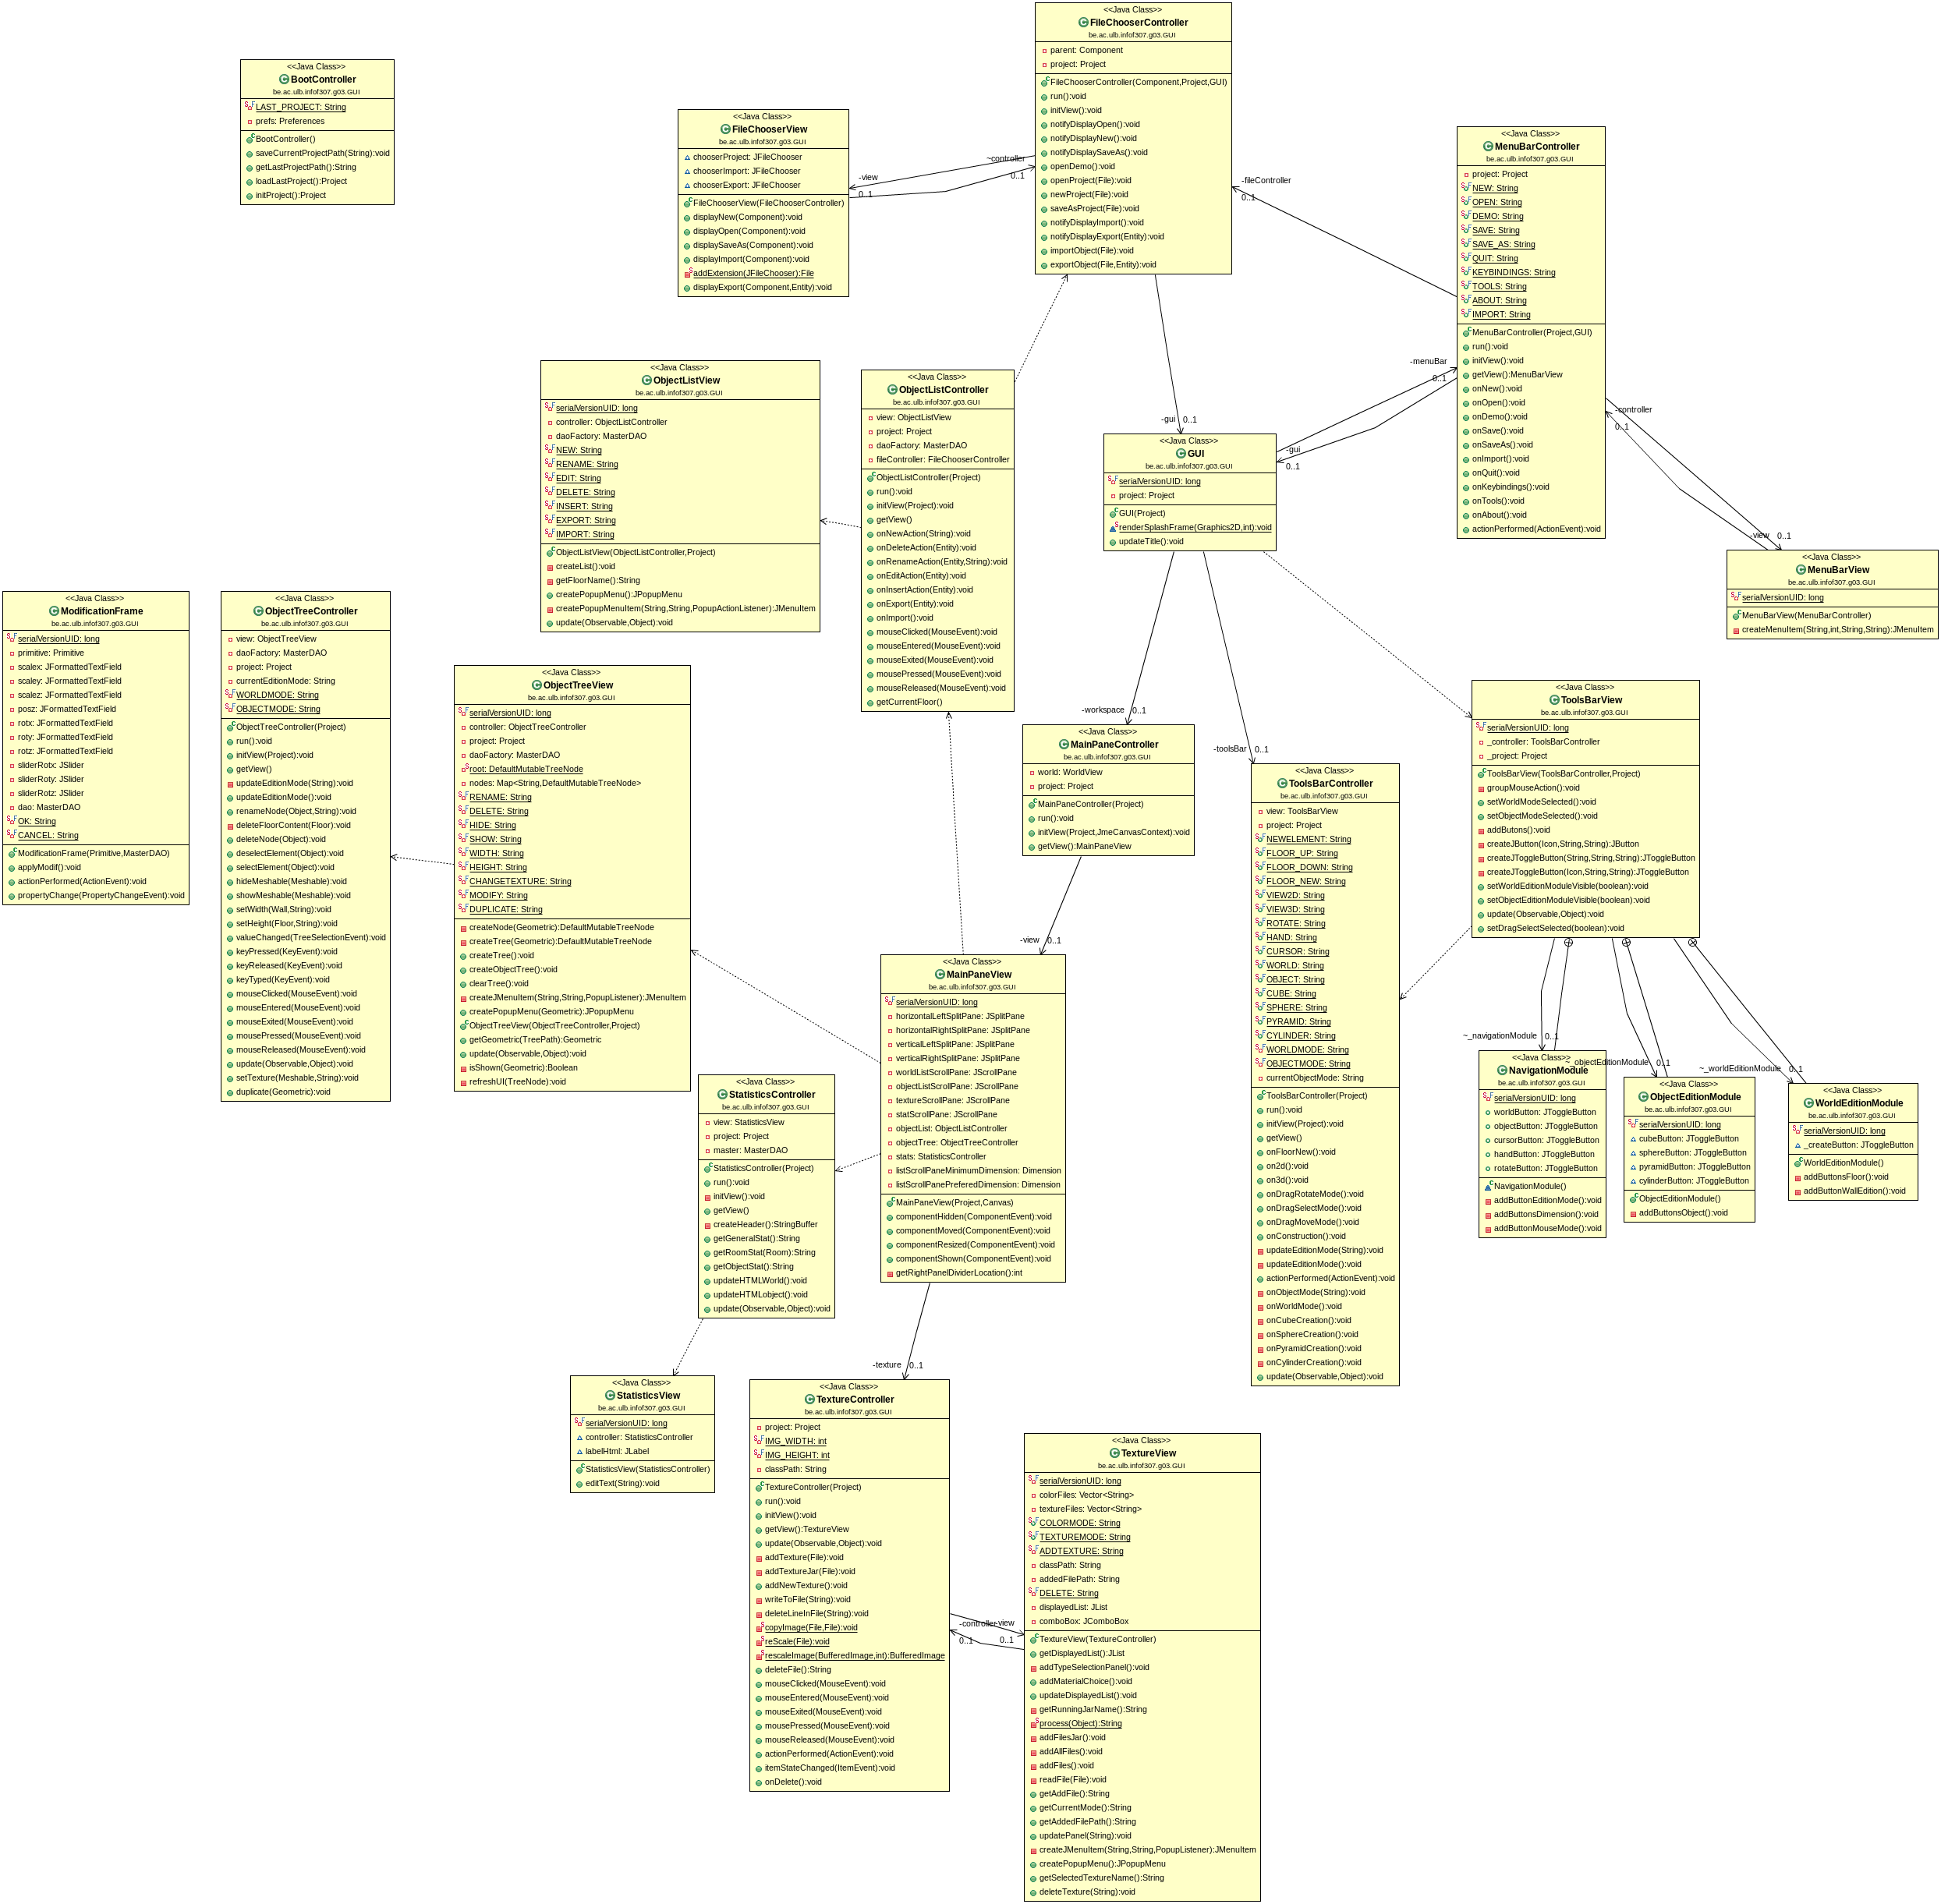
\includegraphics[width=\textwidth]{iteration4/fig/gui-final.png}
	\end{figure}

	\subsubsection{Package io.exporter}
	\begin{figure}[!H]
		\center
		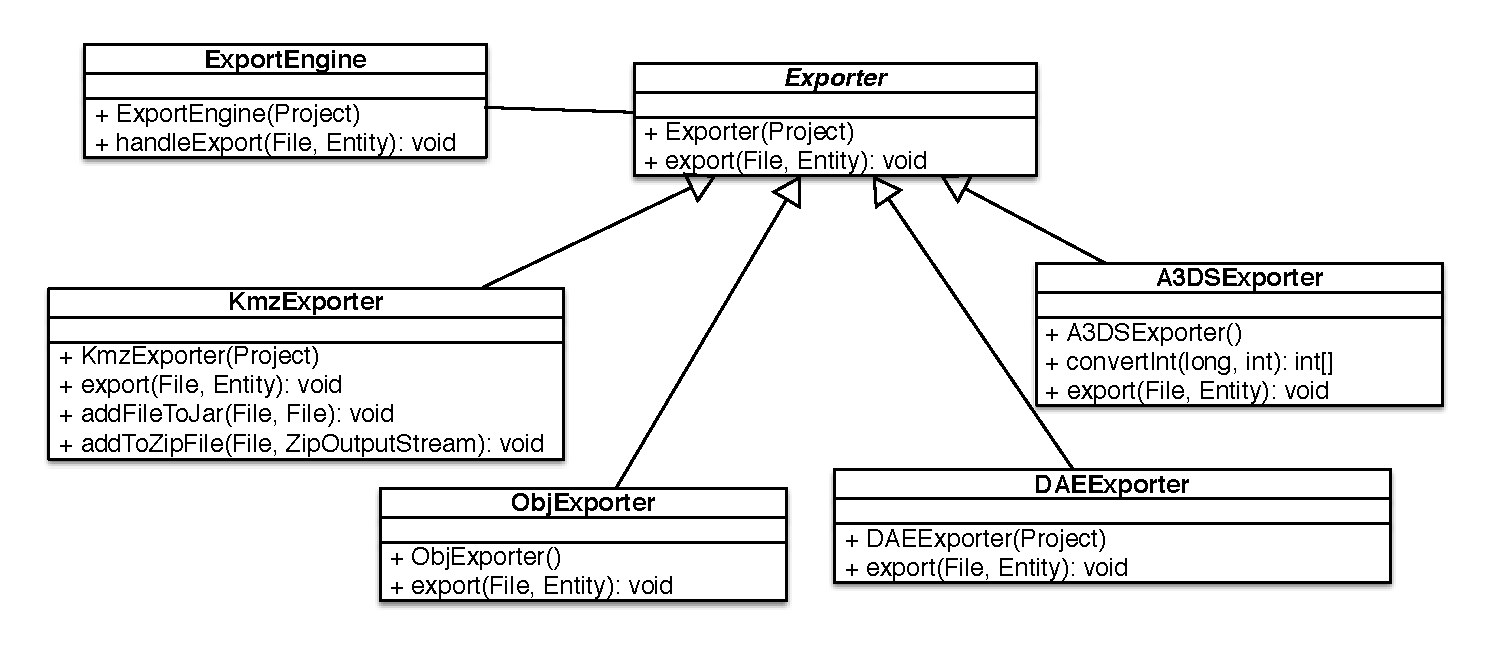
\includegraphics[width=\textwidth]{iteration4/fig/exportfactory.eps}
	\end{figure}

	\subsubsection{Package io.importer}
	\begin{figure}[!H]
		\center
		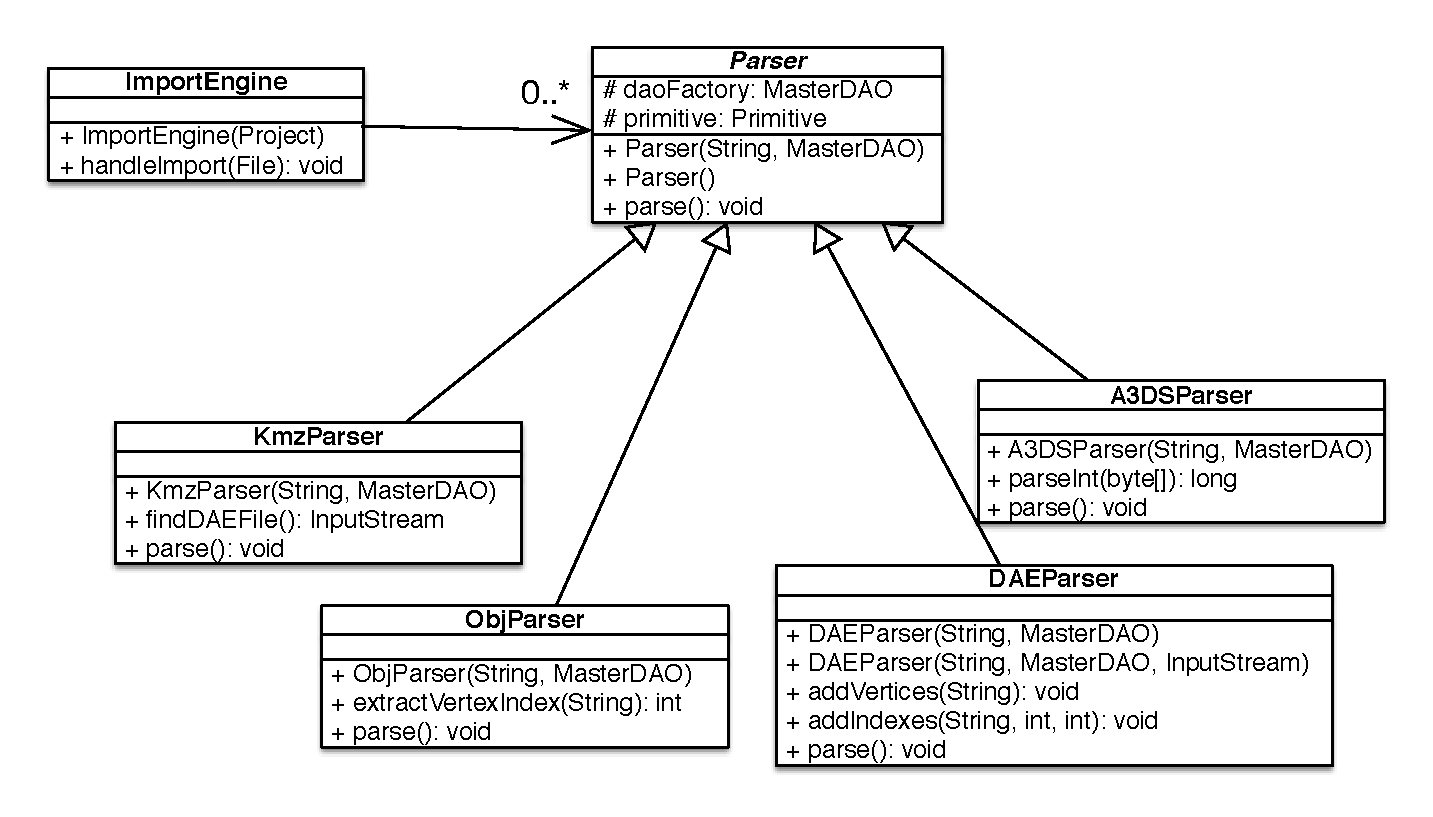
\includegraphics[width=\textwidth]{iteration4/fig/ParsersArchi.eps}
	\end{figure}

	\subsubsection{Package Camera}
	\begin{figure}[!H]
		\center
		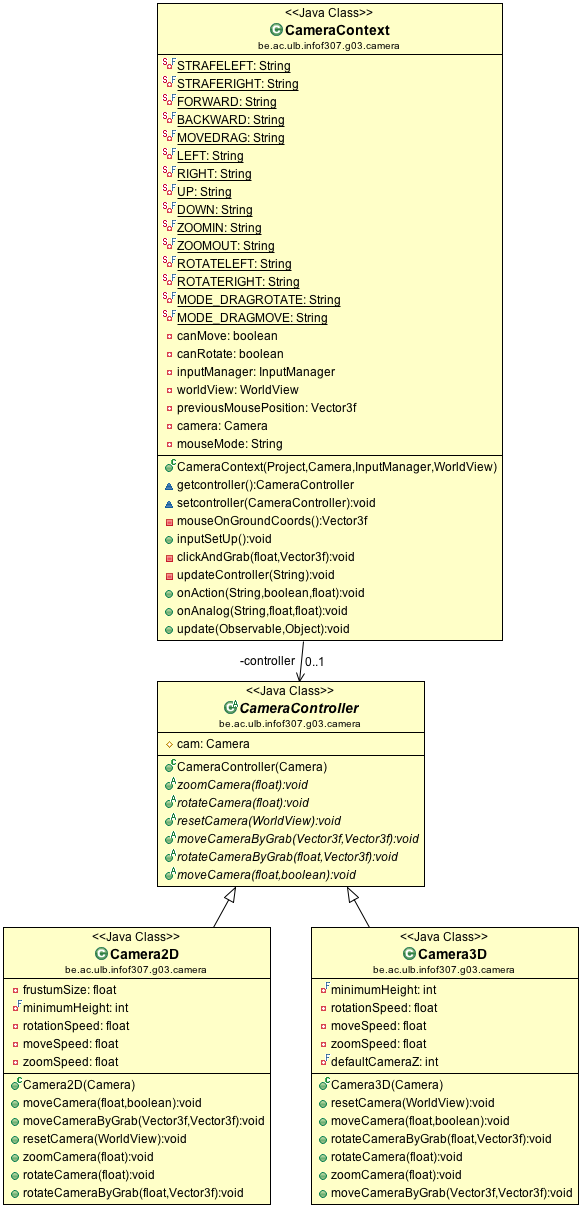
\includegraphics[width=\textwidth]{iteration4/fig/camera.png}
	\end{figure}

	\subsubsection{Package World}
	\begin{figure}[!H]
		\center
		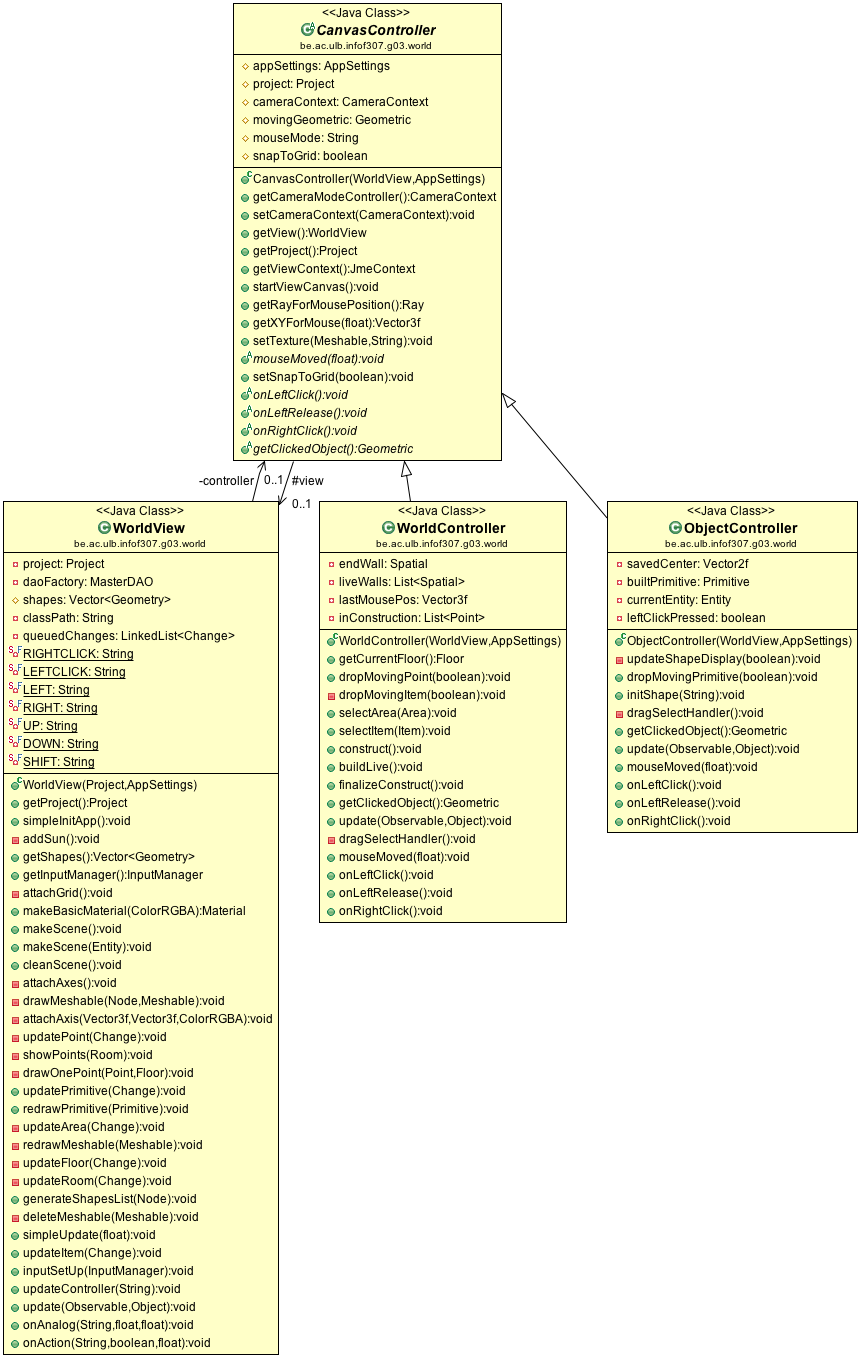
\includegraphics[width=\textwidth]{iteration4/fig/world.png}
	\end{figure}

\subsection{Conclusion}
C'est avec un honneur non dissimulé que je me prête à écrire les quelques
dernières lignes qui représentent la vulgarisation de nos constructions logicielles.
Ces quatre itérations, déroulées dans une franche camaraderie, nous ont permis
à tous de nous épanouir et de grandir dans le travail d'équipe.

Plutôt que de m'étendre dans de longs verbiages peu productifs, je me contenterai
dès lors d'exprimer un sentiment qui nous traverse tous : 

Tout s'est bien passé.
